\documentclass{article}

\usepackage{tikz}
\begin{document}

%\def\input_layer{1}
%\def\hidden_layer_0{5}

\def\hdist{2}

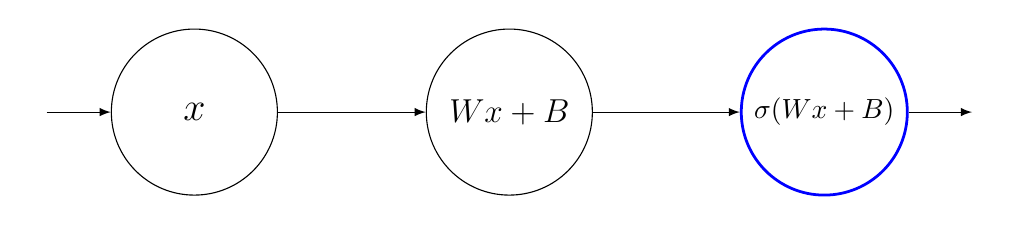
\begin{tikzpicture}

\node (left_input) at (-2, 0) {};
\node[draw, circle, minimum size=60pt] (input) at (0, 0) {\Large $x$};
\draw[->,>=latex] (left_input) -- (input);



% plot the second layer
\node[draw,circle, minimum size=60pt] (output) at (4,0) {\large $Wx+B$};
\draw[->, >=latex] (input) -- (output);


%plot sigmoid
\node[draw , circle , minimum size=60pt , draw=blue, line width=1pt] (sigmoid) at (8,0) {$\sigma(Wx+B)$};
\draw[->, >=latex] (output) -- (sigmoid);

\node (outter) at (10,0) {};
\draw[->, >=latex] (sigmoid) -- (outter);

\end{tikzpicture}

\vspace{150pt}

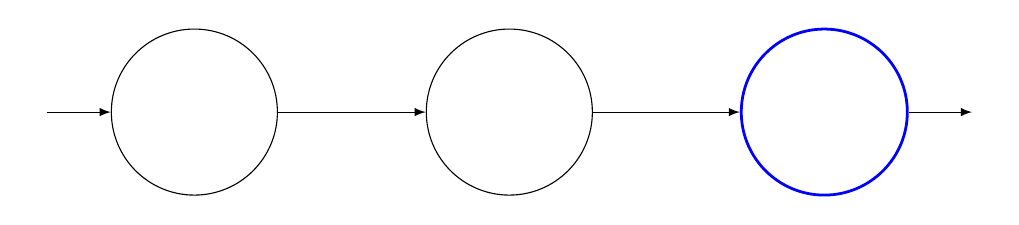
\begin{tikzpicture}

\pgfmathsetmacro\x{0}

\node (left_input) at (\x, 0) {};
\node[draw, circle, minimum size=60pt] (input) at (\x+2, 0) {};
\draw[->,>=latex] (left_input) -- (input);

\pgfmathsetmacro\x{\x+6}



% plot the second layer
\node[draw,circle, minimum size=60pt] (output) at (\x,0) {};
\draw[->, >=latex] (input) -- (output);

\pgfmathsetmacro\x{\x+4}

%plot sigmoid
\node[draw , circle , minimum size=60pt , draw=blue, line width=1pt] (sigmoid) at (\x,0) {};
\draw[->, >=latex] (output) -- (sigmoid);
\node (outter) at (\x + 2,0) {};
\draw[->, >=latex] (sigmoid) -- (outter);

\end{tikzpicture}


% \node[draw , circle ,double, minimum size=60pt, draw=blue, line width=1pt] (sigmoid) at (8,0) {$\sigma(Wx+B)$};
% \node[draw,circle, minimum size=60pt] (output) at (4,0) {\large $Wx+B$};

\end{document}